\subsection{UC6 - Visualizza dettagli file}
\label{UC6}
\begin{figure}[H]
    \centering
    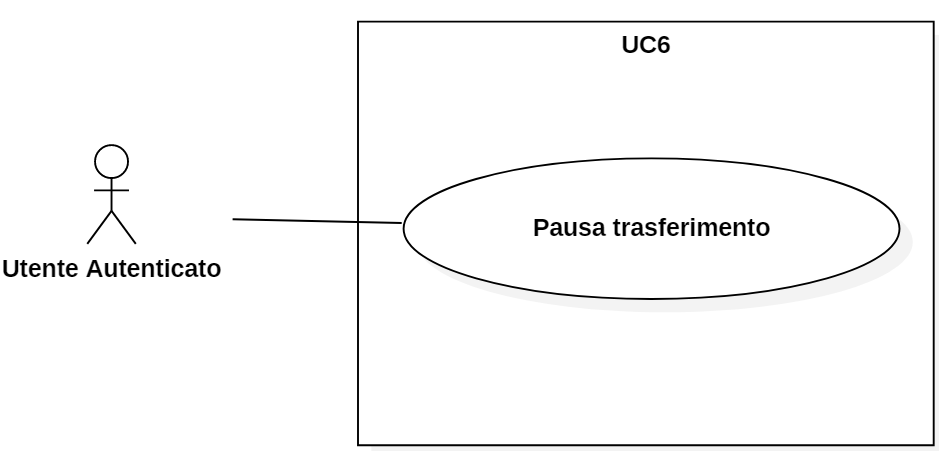
\includegraphics[scale = 0.6]{components/img/UC6.png}
    \caption{UC6 - Visualizza dettagli file}
\end{figure}
\begin{itemize}
\item \textbf{Attore Primario:} Utente autenticato;
\item \textbf{Precondizione:} L'utente ha selezionato la cartella root e sono presenti file al suo interno;
\item \textbf{Postcondizione:} L'utente ha informazioni riguardo al file;
\item \textbf{Scenario principale:} L'utente può visualizzare le informazioni riguardanti i file all'interno della cartella root selezionata.
\end{itemize}

\subsubsection{UC6.1 - Visualizza data creazione file}
\label{UC6.1}
\begin{itemize}
\item \textbf{Attore Primario:} Utente autenticato;
\item \textbf{Precondizione:} L'utente ha selezionato la cartella root e sono presenti file al suo interno;
\item \textbf{Postcondizione:} L'utente è informato sulla data di creazione del file;
\item \textbf{Scenario principale:} L'utente può visualizzare la data di creazione dei file.
\end{itemize}

\subsubsection{UC6.2 - Visualizza data ultima modifica file}
\label{UC6.2}
\begin{itemize}
\item \textbf{Attore Primario:} Utente autenticato;
\item \textbf{Precondizione:} L'utente ha selezionato la cartella root e sono presenti file al suo interno;
\item \textbf{Postcondizione:} L'utente è informato sulla data di ultima modifica del file;
\item \textbf{Scenario principale:} L'utente può visualizzare la data di ultima modifica dei file.
\end{itemize}

\subsubsection{UC6.3 - Visualizza grandezza file}
\label{UC6.3}
\begin{itemize}
\item \textbf{Attore Primario:} Utente autenticato;
\item \textbf{Precondizione:} L'utente ha selezionato la cartella root e sono presenti file al suo interno;
\item \textbf{Postcondizione:} L'utente è informato sulla grandezza del file;
\item \textbf{Scenario principale:} L'utente può visualizzare la grandezza dei file.
\end{itemize}

\subsubsection{UC6.4 - Visualizza stato dei file}
\label{UC6.4}
\begin{itemize}
\item \textbf{Attore Primario:} Utente autenticato;
\item \textbf{Precondizione:} L'utente ha effettuato dei trasferimenti da o verso il server;
\item \textbf{Postcondizione:} L'utente è informato sullo stato dei file sincronizzati e non;
\item \textbf{Scenario principale:} L'utente può visualizzare lo stato corrente dei file.
\end{itemize}